\chapter{Introduction}
\label{chapter1}

Motivate the research in probabilistic models.

\section{Motivations}
\label{section1.1}

Most tasks conducted by a person or an automated system requires a fundamental ability of \textit{reasoning}, which is always about reaching a conclusion based on available information. At times, a conclusion is not enough and it is also required to know how reliable the conclusion is. Take the coronavirus that started from Wuhan, China at the end of 2019, as example, a doctor needs checks the information about a person to reason if the person is infected by the coronavirus. The relevant information includes symptoms such as fever, cough, breathing difficulties and probably kidney failure in severe cases. \textcolor{red}{maybe a small figure of coronavirus here}. Even after the doctor has concluded as positive or negative of ccoronavirus for the person, the natural question is why and how \textit{confident} the diagnose is.

\begin{example}
  coronavirus
\end{example}

\begin{example}
  digital communication? Y, X
\end{example}

Two problems are inevitable to conduct the reasoning:
\begin{itemize}
\item How should we specify the relationship between a conclusion and the available information? In the coronavirus example, the counterpart question to answer is how the doctor should relate coronavirus infection with the symptoms. This step is called \textit{modeling} which represents a reasoning problem abstractly by specifying the relationship between known information and unknown part, in preparation of answer query on it.
\item With the model, how a conclusion should be made? This process of reaching a answer to the query is called \textit{inference}. \textcolor{red}{something about coronavirus}
\end{itemize}

As times, a model is not totally fixed since one may not be sure the correctness of the assumptions about the model. A typical strategy is to leave some freedom in the configuration of the model at beginning. By using previous observations or information, the model is adjusted to be able to explain the observation in more reasonable way. This adds the following problem in reasoning:
\begin{itemize}
  \item Instead of having a fixed model at the first step, a set of model is given. We then need to choose one model based previous observations to do inference in order to make conclusion or answer query. This phase of choosing a model is called \textit{learning}.
\end{itemize}

With all the discussed problems above, modelling, inference and learning, our purpose is to carry out reasoning with being aware of how confident a conclusion or answer is. 
These problems can be treated nicely with probabilistic models. Probabilistic models is built on the fundamental calculus of probability theory that is natural to accommodate the \textit{uncertainty}, which is desired in reasoning. In additional, the probabilistic models offers rich space to modeling problems, where inference can be carried on either exactly or approximately. \textbf{More importantly, the modeling or modeling learning part is not necessarily coupled with inference algorithm.} This proper separation allows free that a certain family of general inference algorithms can be applies to a broad class probabilistic models. It offers the freedom of trying different models of a class without the need of replacing inference algorithm. 


Back to the example of coronavirus, we are able to model the problem and also the query more formally in probabilistic model framework. For instance, assume each symptom among fever, cough and breathing difficulty can take value from $\left\{ \mathrm{True}, \mathrm{False} \right\}$. Also the coronavirus infection is either true or false. One exemplified query can be
\begin{equation}
  P(\mathrm{Infection} = \mathrm{True} | \mathrm{Fever} = \mathrm{True}, \mathrm{Cough} = \mathrm{False}, \mathrm{Breathing Difficulty}= \mathrm{True}), \nonumber
\end{equation}
which is asking how likely the patient is infected by coronavirus if symptoms of both fever and breathing difficulty are observed but no sight of cough.
\begin{figure}[!t]
  \centering
  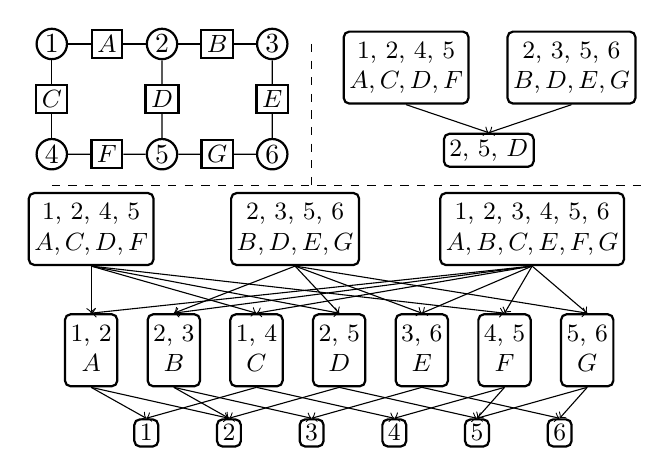
\begin{tikzpicture}
    \begin{scope}[scale=0.7]

    \tikzstyle{cnode} = [thick, draw=black, circle, inner sep = 1pt,  align=center]
    \tikzstyle{nnode} = [thick, rectangle, rounded corners = 0pt,draw,inner sep = 2pt]
    \node[cnode] (x1) at (0,0) {1};
    \node[cnode] (x2) at (2,0) {2};
    \node[cnode] (x3) at (4,0) {3};

    \node[cnode] (x4) at (0,-2) {4};
    \node[cnode] (x5) at (2,-2) {5};
    \node[cnode] (x6) at (4,-2) {6};

    \node[nnode] (fa) at (1,0) {\small$A$};
    \node[nnode] (fb) at (3,0) {\small$B$};

    \node[nnode] (fc) at (0,-1) {\small$C$};
    \node[nnode] (fd) at (2,-1) {\small$D$};
    \node[nnode] (fe) at (4,-1) {\small$E$};
        
    \node[nnode] (ff) at (1,-2) {\small$F$};
    \node[nnode] (fg) at (3,-2) {\small$G$};


    \draw[-] (x1) -- (fa);
    \draw[-] (x1) -- (fc);

    \draw[-] (x2) -- (fa);
    \draw[-] (x2) -- (fb);
    \draw[-] (x2) -- (fd);

    \draw[-] (x3) -- (fb);
    \draw[-] (x3) -- (fe);

    \draw[-] (x4) -- (fc);
    \draw[-] (x4) -- (ff);

    \draw[-] (x5) -- (fd);
    \draw[-] (x5) -- (ff);
    \draw[-] (x5) -- (fg);

    \draw[-] (x6) -- (fe);
    \draw[-] (x6) -- (fg);

    \end{scope}
    \draw[dashed] (0, -1.8) -- (7.5, -1.8) (3.3, 0) -- (3.3, -1.8);
    
    \begin{scope}[xshift=4.5cm, yshift=-0.3cm,scale=0.7]
      \tikzstyle{rnode} = [thick, rectangle, rounded corners = 2pt,minimum size = 0.0cm,draw,inner sep = 2pt]
      \node[rnode] (r01) at (0,0) {\small \begin{tabular}[x]{@{}c@{}}1, 2, 4, 5 \\ $A,C,D,F$ \end{tabular}};
      \node[rnode] (r02) at (3,0) {\small \begin{tabular}[x]{@{}c@{}}2, 3, 5, 6\\ $B,D,E,G$ \end{tabular}};
      \node[rnode] (r11) at (1.5, -1.5) {\small 2, 5, $D$};

      \draw[->] (r01.south) -- (r11.north);
      \draw[->] (r02.south) -- (r11.north);

    \end{scope}

    \begin{scope}[xshift=0.5cm, yshift=-2.35cm,scale=0.7]
      \tikzstyle{rnode} = [thick, rectangle, rounded corners = 2pt,minimum size = 0.0cm,draw,inner sep = 2pt]
      \node[rnode] (r01) at (0,0) {\small\begin{tabular}[x]{@{}c@{}}1, 2, 4, 5 \\ $A,C,D,F$ \end{tabular}};
      \node[rnode] (r02) at (3.7,0) {\small\begin{tabular}[x]{@{}c@{}}2, 3, 5, 6\\ $B,D,E,G$ \end{tabular}};
      \node[rnode] (r03) at (8,0) {\small\begin{tabular}[x]{@{}c@{}}1, 2, 3, 4, 5, 6\\ $A,B,C,E,F,G$ \end{tabular}};
      \begin{scope}[yshift=-0.2cm]
      \node[rnode] (r11) at (0, -2.0) {\small\begin{tabular}[x]{@{}c@{}}1, 2\\ $A$ \end{tabular}};
      \node[rnode] (r12) at (1.5, -2.0) {\small\begin{tabular}[x]{@{}c@{}}2, 3\\ $B$ \end{tabular}};
      \node[rnode] (r13) at (3, -2.0) {\small\begin{tabular}[x]{@{}c@{}}1, 4\\ $C$ \end{tabular}};
      \node[rnode] (r14) at (4.5, -2.0) {\small\begin{tabular}[x]{@{}c@{}}2, 5\\ $D$ \end{tabular}};
      \node[rnode] (r15) at (6, -2.0) {\small\begin{tabular}[x]{@{}c@{}}3, 6\\ $E$ \end{tabular}};
      \node[rnode] (r16) at (7.5, -2.0) {\small\begin{tabular}[x]{@{}c@{}}4, 5\\ $F$ \end{tabular}};
      \node[rnode] (r17) at (9, -2.0) {\small\begin{tabular}[x]{@{}c@{}}5, 6\\ $G$ \end{tabular}};

      \begin{scope}[yshift=0.5cm]
      \node[rnode] (r21) at (1, -4) {\small 1};
      \node[rnode] (r22) at (2.5, -4) {\small 2};
      \node[rnode] (r23) at (4, -4) {\small 3};
      \node[rnode] (r24) at (5.5, -4) {\small 4};
      \node[rnode] (r25) at (7, -4) {\small 5};
      \node[rnode] (r26) at (8.5, -4) {\small 6};
      \end{scope}
      \end{scope}
      % edge level0 to level1
      \draw[->] (r01.south) -- (r11.north);
      \draw[->] (r03.south) -- (r11.north);

      \draw[->] (r02.south) -- (r12.north);
      \draw[->] (r03.south) -- (r12.north);

      \draw[->] (r01.south) -- (r13.north);
      \draw[->] (r03.south) -- (r13.north);

      \draw[->] (r01.south) -- (r14.north);
      \draw[->] (r02.south) -- (r14.north);

      \draw[->] (r02.south) -- (r15.north);
      \draw[->] (r03.south) -- (r15.north);

      \draw[->] (r01.south) -- (r16.north);
      \draw[->] (r03.south) -- (r16.north);

      \draw[->] (r02.south) -- (r17.north);
      \draw[->] (r03.south) -- (r17.north);

      % edge level1 to level2
      \draw[->] (r11.south) -- (r21.north);
      \draw[->] (r13.south) -- (r21.north);

      \draw[->] (r11.south) -- (r22.north);
      \draw[->] (r12.south) -- (r22.north);
      \draw[->] (r14.south) -- (r22.north);


      \draw[->] (r12.south) -- (r23.north);
      \draw[->] (r15.south) -- (r23.north);

      \draw[->] (r13.south) -- (r24.north);
      \draw[->] (r16.south) -- (r24.north);

      \draw[->] (r14.south) -- (r25.north);
      \draw[->] (r16.south) -- (r25.north);
      \draw[->] (r17.south) -- (r25.north);

      \draw[->] (r15.south) -- (r26.north);
      \draw[->] (r17.south) -- (r26.north);
    \end{scope}
  \end{tikzpicture}
  \vskip -0.15in
  \caption{Illustration of a factor graph for 2-by-3 grid (top left, variable nodes are indexed by number and factor nodes by letters), and two alternative regions graphs (two levels for the top right one and three levels for bottom one) constructed from the factor graph.}
  \label{fig:factor-region-graphs}
  \vskip -0.2in
\end{figure}
basic problems: 1. modeling, 2. inference, 3. learning?

what graphical models do and why

what learning means


the inference diagram here


the learning diagram here
\begin{itemize}
\item Structural learning
\item parameter learning
\end{itemize}


the learning principle:
\begin{itemize}
 \item Maximal likelihood estimation (MLE)
\item Bayesian estimation
\item Maximal conditional likelihood
\item Maximal '' `Margin`''
\item Maximum entropy
\end{itemize}



\section{Scope and Thesis Outline}

\subsection{Summary of Contributions}
\cite{liu2019dominant}

\subsection{Publications}

Tools (code) developed:


%%% Local Variables:
%%% mode: latex
%%% TeX-master: "../../main"
%%% End:
